%!TEX root = ../report.tex

% 
% Related work
% 
% (~17pgs)
\section{Related Work}

% começar por dizer como é que está organizada esta secção do trabalho e resumir de uma forma muito geral o que se fala em cada subsecção

This section presents the related work for this project and characterizes the main contributions of past works and how these contributions helped in the development of this project. This section is organized is the main parts: mHealth, mobile security and TrustZone.

The first part focuses on describing the attack surfaces of mHealth apps, the most common threats and their seriousness, present a few publicly available unsecure mHealth apps as well as some compliance recommendations that app developers should follow to avoid unnecessary security risks when handling sensitive health information. The second part of this sections describes the state of the art of mobile security with a particular focus on the Android Operating System and how developers can build secure applications with a trusting \ac{OS} and security mechanisms built upon the application layer. The third part of the related work describes TrustZone, a hardware technology available a most modern \ac{ARM} processors which supports executions of two isolated worlds, a hardware secure world and a normal world. Besides describing the technology this sections also presents previous work developed using TrustZone and who these previous contributions may be helpful in achieving the main goals of this project. 

\subsection{mHealth}

As discussed above, mobile devices are increasing in number at astonishing rates and with this growth the mobile market becomes cheap and accessible. This motivates the shift from mainframe systems located in the facilities of healthcare providers to apps on mobile devices as well as storage in shared could services. This accessibility also motivates the private sector in building more healthcare applications to support both patients and healthcare agents. Thus, the mobile health market is becoming a competitive market and one which is increasingly handling with more sensitive data.

Kotz, David \cite{kotz2011threat} defines a threat taxonomy for mHealth. He, Dongjing, et al. \cite{he2014security} analyse several mHealth applications available in Android's app store considering the most common attack surfaces, shown in table \ref{tab:attacksurfaces}. This work contributes with understanding of security and privacy risk on the Android platform.

\begin{table}
	\caption {Description of attack surface}
	\label{tab:attacksurfaces}
	\begin{tabular}{|>{\raggedright}p{2cm}|>{\raggedright\arraybackslash}p{10cm}|}
		\hline
		\textbf{Attack Surface}      & \textbf{Description}                                                                                                                    \\ \hline
		Internet            & Sensitive information is sent over the internet with unsecure protocols (e.g. HTTP), misconfigured HTTPS, etc.                 \\ \hline
		Third Party         & Sensitive information is stored in third party servers                                                                         \\ \hline
		Bluetooth           & Sensitive information collected by Bluetooth-enabled health devices can be sniffed or injected                                 \\ \hline
		Logging             & Sensitive information is put into system logs where it is not secured                                                          \\ \hline
		SD Card Storage     & Sensitive information is stored as unencrypted files on SD card, publicly accessible by any other app                          \\ \hline
		Exported Components &  Android app components, intended to be private, are set as exported, making them accessible by other apps                     \\ \hline
		Side Channel        & Sensitive information can be inferred by a malicious app with side channels, e.g. network package size, sequence, timing, etc. \\ \hline
	\end{tabular}
\end{table}
\FloatBarrier

%\subsection{Mobile Security}
%
%TEXT HERE\\
%TEXT HERE\\
%TEXT HERE
%
%\subsection{TrustZone}
%
%TEXT HERE\\
%TEXT HERE\\
%TEXT HERE
%
%\subsubsection*{Andix OS\\}
%TEXT HERE\\
%TEXT HERE\\
%TEXT HERE

%% Example citation:
%THIS IS A CITATION\cite{Braem2013a}
%
%The related work section will highly volatile, and will mostly depend on your kind of thesis. Talk with your supervisor in order to know how to write this part. Don't take the following bullet points as a certain truth.
%
%\begin{itemize}
%  \item Most important part of the document. Might be divided in 2/3 subsections.
%  \item Might be devised into related work and 
%  \item Should cite a wide range of references ~30, search in google, google scholar, mendley, IEEE explorer etc..
%  \item Summarized table of solutions.
%\end{itemize}
%
%Citations should be mostly :
%\begin{itemize}
%  \item magazine articles
%  \item conferences / workshops
%  \item books and technical reports
%\end{itemize}
%And make sure that your citations follow the following criteria:
%\begin{itemize}
%  \item Conferences: name and year
%  \item workshops: name of the workshop, name of the conference, location and year
%  \item Magazines: volume, issue (if possible article pages), publisher.
%  \item Books: title, publisher, ISBN, year
%\end{itemize}
%Websites should be added as footnotes~\footnote{www.google.com}
%
% Example image:
%\begin{figure}[hb!]
%  \centering
%  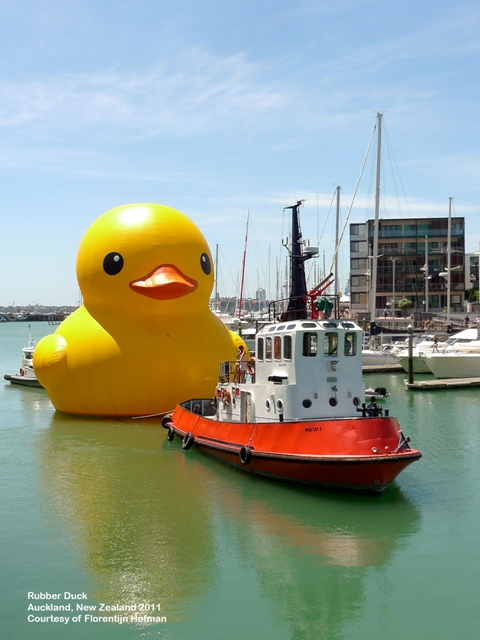
\includegraphics[width=0.95\textwidth]{img/rubberduck.jpg}
%  \caption{caption}
%  \label{fig:label}
%\end{figure}





